\section{Controller design} \label{sec:ctrl-design}
This chapter firstly presents the basic LQR and LQI controller theory and secondly the derived controller. 

\subsection{Linear-Quadratic Regulator} \label{sec:ctrl_lqr}
The Linear-Quadratic Regulator (LQR) in its \textit{infinite horizon} form is the preferred controller. It is chosen because the LQR tuning process of choosing weights to penalize state deviations is deemed more intuitive than defining pole locations in the \textit{pole placement method}. Furthermore an LQR controller guarantees 6 dB gain margin and 60 degree phase margin \cite{Doyle1978}. 

For a system
\begin{equation}\label{eq:ctrl_sys}
	\begin{split}
		\dot x &= A x + B u \\
		y &= Cx
	\end{split}
\end{equation}
the LQR controller is an optimal with respect to a relevant cost function such as:
\begin{equation}\label{eq:lqr_cost}
	J = \int_{0}^{\infty} \left(x^T Q x + u^T R u + 2x^T N u\right) dt
\end{equation}
where
\begin{center}
	\begin{tabular}{l r l }
		weight & $R$         & $ > 0$ (positive definite) and symmetric       \\
		weight & $Q$ and $N$ & $\ge 0$ (positive semi-definite) and symmetric
	\end{tabular}
\end{center}
\smallskip
The final term cross-term which punishes combinations of inputs and states is usually omitted by setting $ N = 0 $. The diagonal entries of $ R $ and $ Q $ are considered tuning parameters. The solution to the LQR control problem is the optimal control feedback which minimizes the cost function. The LQR controller is thus inherently a regulator meaning that it drives the system states to 0. For a system linearised at an operating point $ \{x_o, u_o\} $ the state and input deviations from the operating point replaces the actual states and inputs: $ \hat x = x-x_o $ and $ \hat u = u-u_o $. Given that the operating point is located at the reference the regulator property is obviously not unattractive. With $ N = 0 $ and states substituted with state deviations the final cost function becomes:
\begin{equation}\label{eq:lqr_cost_final}
	J = \int_{0}^{\infty} \left(\hat x^T Q \hat x + \hat u^T R \hat u\right) dt
\end{equation}
The optimal feedback gain can be shown to be: 
\begin{equation}\label{eq:lqr_K}
	K = -R^{-1} B^T P
\end{equation}
with P being the solution to the algebraic Ricatti equation:
\begin{equation}\label{lqr:ricatti}
	A^T P + P A - P B R^{-1} B^T P + Q = 0
\end{equation}
This leaves $ Q $ and $ R $ to be tuned in such a manner that a satisfactory performance is achieved. For initial guesses \textit{Bryson's Rule} can be utilized. It states that a diagonal entry in $ Q $ or $ R $ for a corresponding state $ x_i $ or input $ u_i $ should be set as such:
\begin{equation}\label{eq:bryson}
	\begin{split}
		Q_i = \dfrac{1}{Max(\hat x_i)^2} \\
		R_i = \dfrac{1}{Max(\hat u_i)^2}
	\end{split}
\end{equation}
where $ Max(\hat x) $ is the largest tolerated value of $ \hat x $. While optimal performance is rarely achieved without further tuning Bryson's Rule gives a good starting point. In Matlab the \textit{lqr(A, B, Q, R, N)} function is used to get the controller gains $ K $.


\subsection{Linear-Quadratic Integrator} \label{sec:ctrl_lqi}
As described \cref{sec:comp_flc} the FLC controller is of the proportional-integrator (PI) type which ensures no generator speed steady state error due to integral action. The controller to be derived includes generator speed control and the regular LQR controller does not have integral action. Therefore the system is augmented with an integral state on the generator speed $ \dot x_i = \hat \omega $ leaving the extended state space system to be:
\begin{align} 
	\dot {\bar x} & = \begin{bmatrix} \dot{\hat x} \\ \dot x_i \end{bmatrix} = \begin{bmatrix} A &0 \\ C_{iy} & 0 \end{bmatrix} \bar x + \begin{bmatrix} B_u \\ 0 \end{bmatrix}  \hat u \\
	\hat y & = \begin{bmatrix} C & 0 \end{bmatrix} \bar x
\end{align}
where $ C_{iy} $ is defined such that the output to be integrated is picked out and $ \bar x $ is the deviation state vector extended with the integral state. %; in this case the generator speed.

A linear quadratic integrator (LQI) controller is obtained when the integrator-augmented system matrices are used to solve the LQR problem. The dimension of $ Q $ increases for every extra integrator state and thus extra weights are defined for these. 


\subsection{The controller} \label{sec:ctrl_thecontroller}
In the preceding sections the LQR and LQI controllers were explained and we are therefore ready to make the LQI controller. Firstly the FLC controller is removed from the system such that the input to the system is the pitch reference $ thRef $ in stead of the rotor speed reference $ wRef $. Stability and controllability are checked and the system is both stable and controllable. The \textit{lqr()} matlab function is used with the integrator-augmented system. Bryson's Rule is used to define $ Q $ and $ R $ by defining maximum limits to the states and controllable inputs. A less intuitive weight is put on the integrator state. After a controller tuning process the resulting gains are:
\begin{equation}\label{eq:lqi_K}
	K = \begin{bmatrix} -1.264 &  1.249 & -75.159 & -9.549 \end{bmatrix}
\end{equation}
when the $ Q $ and $ R $ matrices are defined as such:
\begin{equation}\label{eq:lqi_Q_and_R}
	\begin{split}
		Q = \begin{bmatrix}
			\dfrac{1}{max(p_y)^2}& 0 					& 0 															& 0 \cr
			0 					& \dfrac{1}{max(v_y)^2}	& 0 															& 0 \cr
			0 					& 0 					& \dfrac{1}{\left( max(\Omega) \cdot \frac{2 \pi}{60} \right)^2} & 0 \cr
			0 					& 0 					& 0 															& \dfrac{1}{(max(\Omega_i) \cdot \frac{2 \pi}{60})^2} \end{bmatrix} & = \begin{bmatrix}
			\dfrac{1}{5^2} 	&  	0 				&  0 										&  0 \cr
			0 				&  \dfrac{1}{1^2}	&  0 										&  0 \cr
			0 				&  0 				& \dfrac{1}{\left( 1 \cdot \frac{2 \pi}{60} \right)^2} 	&  0 \cr
			0 				&  0 				&  0 										&  \dfrac{1}{(5 \cdot \frac{2 \pi}{60})^2}
		\end{bmatrix} \\\\
		R = \begin{bmatrix} \dfrac{1}{\max(\theta_{ref})^2} \end{bmatrix} &= \begin{bmatrix} \dfrac{1}{5^2} \end{bmatrix}
	\end{split}
\end{equation}
From $ Q $ and $ R $ it is observable that:
\begin{itemize}
	\item the maximum allowed fore-aft position deviation is set to 5 m
	\item the maximum allowed fore-aft velocity deviation is set to 1 m/s
	\item the maximum allowed fore-aft rotor speed deviation is set to 1 rpm
	\item the rotor speed integration weight is set 5 times lower than the rotor speed
	\item the maximum allowed pitch angle actuation deviation is set to 5 deg
\end{itemize}
$ 2 \pi $/$ 60 $ is multiplied with the rotor speed tolerances to translate the weight from rad/s to rpm. There is furthermore no intuitive explanation behind the choice of the integrator weight other than that it has yielded satisfactory results in the controller tuning process. Little tuning was necessary from the initial guesses of maximum tolerable state and input values to achieve good performance. This highlights the usefulness of the LQR controller when a fitting linear model is used. Also perhaps importantly when the necessary system understanding has not been achieved such that placement of poles with the pole placement method can be done based on reasonable design considerations. Significant system understanding can be achieved by observing the positions of poles and zeros and thus a drawback of LQR is perhaps that some understanding of the system is lost.
%\begin{equation}\label{eq:lqi_Q_and_R}
%	Q =   \begin{bmatrix}
%		0.04 &  0 &  0 &  0 \cr
%		0 &  1 &  0 &  0 \cr
%		0 &  0 & 91.1 &  0 \cr
%		0 &  0 &  0 &  3.65
%	\end{bmatrix}
%	 \;\; and \;\; 
%	R = \begin{bmatrix} 0.04 \end{bmatrix}
%\end{equation}



%s_W = 1; s_py = 5; s_vy = 1; s_Wi = s_W*5; s_th = 5;
%var_Omega	= (s_W * (2*pi)/60)^2;	% Permitted variance of Omega in [rad/s]
%var_py		= s_py^2;				% Permitted variance of py in [m]
%var_vy		= s_vy^2;				% Permitted variance of vy in [m/s]
%Qlqr = [1/var_py	0			0
%0			1/var_vy	0
%0			0			1/var_Omega];


%\begin{equation}\label{eq:lqi_Q_and_R}
%	Q =   \begin{bmatrix}
%		\dfrac{1}{5^2} 	&  	0 				&  0 										&  0 \cr
%		0 				&  \dfrac{1}{1^2}	&  0 										&  0 \cr
%		0 				&  0 				& \dfrac{1}{\left( 1 \cdot \frac{2 \pi}{60} \right)^2} 	&  0 \cr
%		0 				&  0 				&  0 										&  \dfrac{1}{(5 \cdot \dfrac{2 \pi}{60})^2}
%	\end{bmatrix}
%	\;\; and \;\; 
%	R = \begin{bmatrix} \dfrac{1}{5^2} \end{bmatrix}
%\end{equation}

\subsection{LQI controller tuning analysis}
This section is dedicated to gaining an understand of how the LQI controller moves the system poles when weights are changed. The pole-zero map of the system with no FLC or LQI controller is compared to the system when the LQI controller is applied with varying weights.



% VY
\begin{figure}[ht]
	\centering
	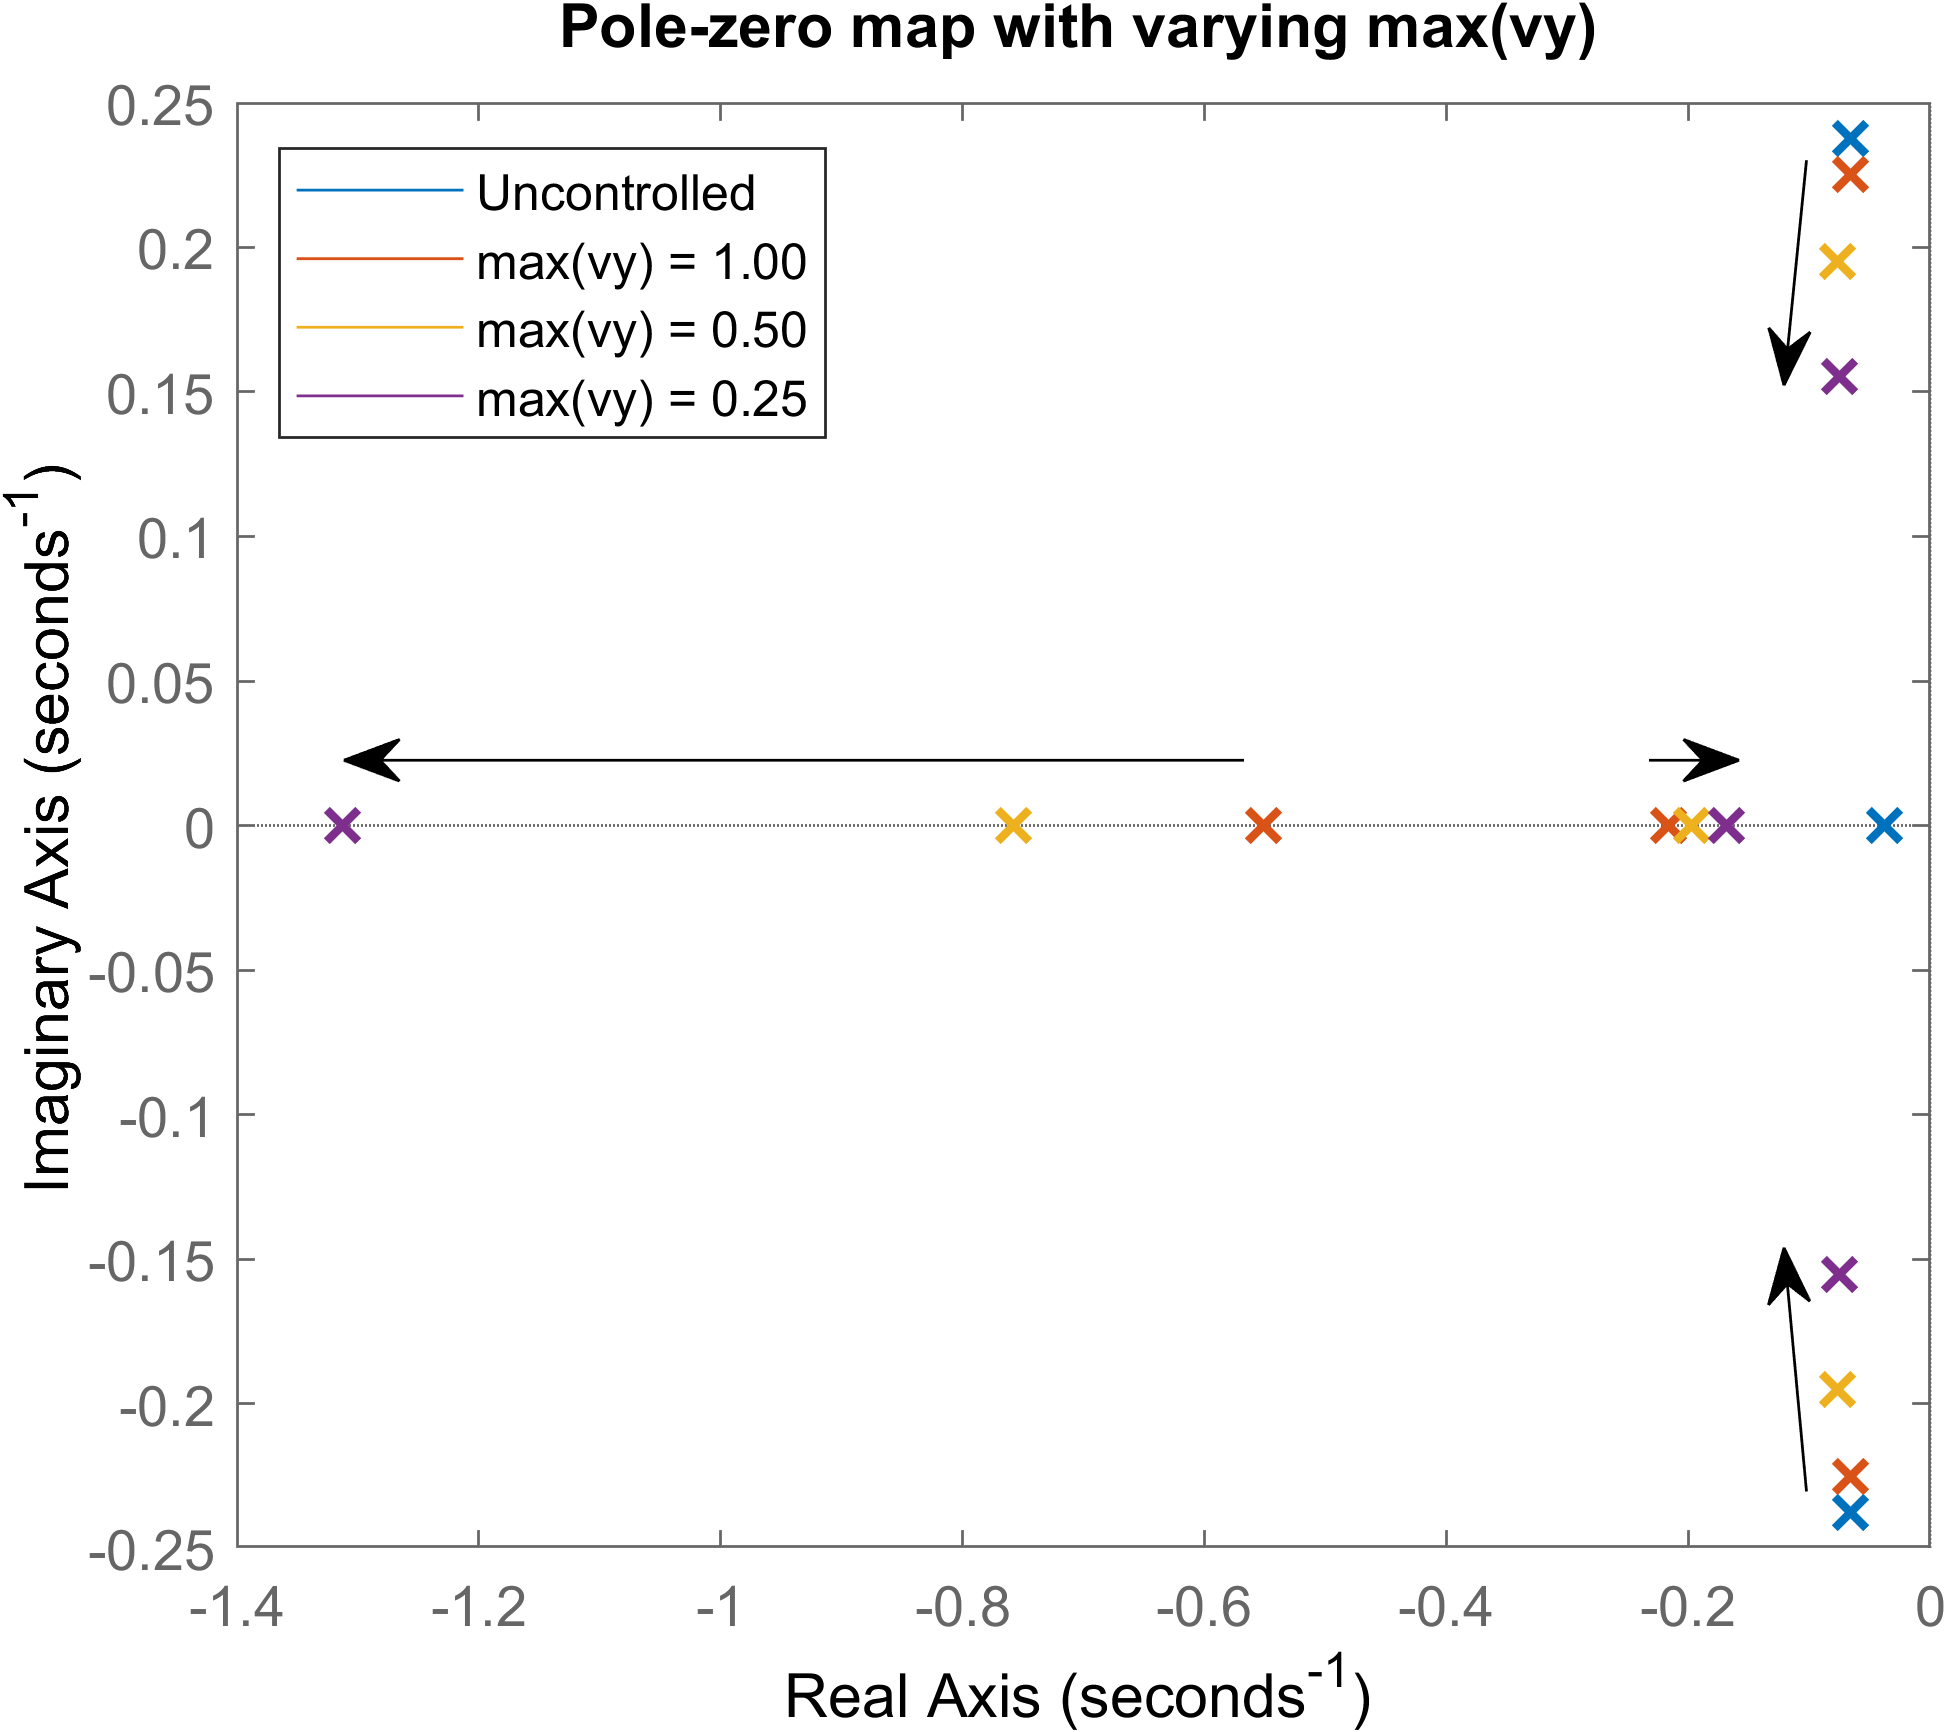
\includegraphics[width=.55\textwidth]{Graphics/LQI pole zero/02_pzmap_vy}
	\caption{Pole-zero diagram with varying LQI weight of the state $ v_y $.}
	\label{fig:pzmap_vy}
\end{figure}


\begin{figure}[ht]
	\centering
	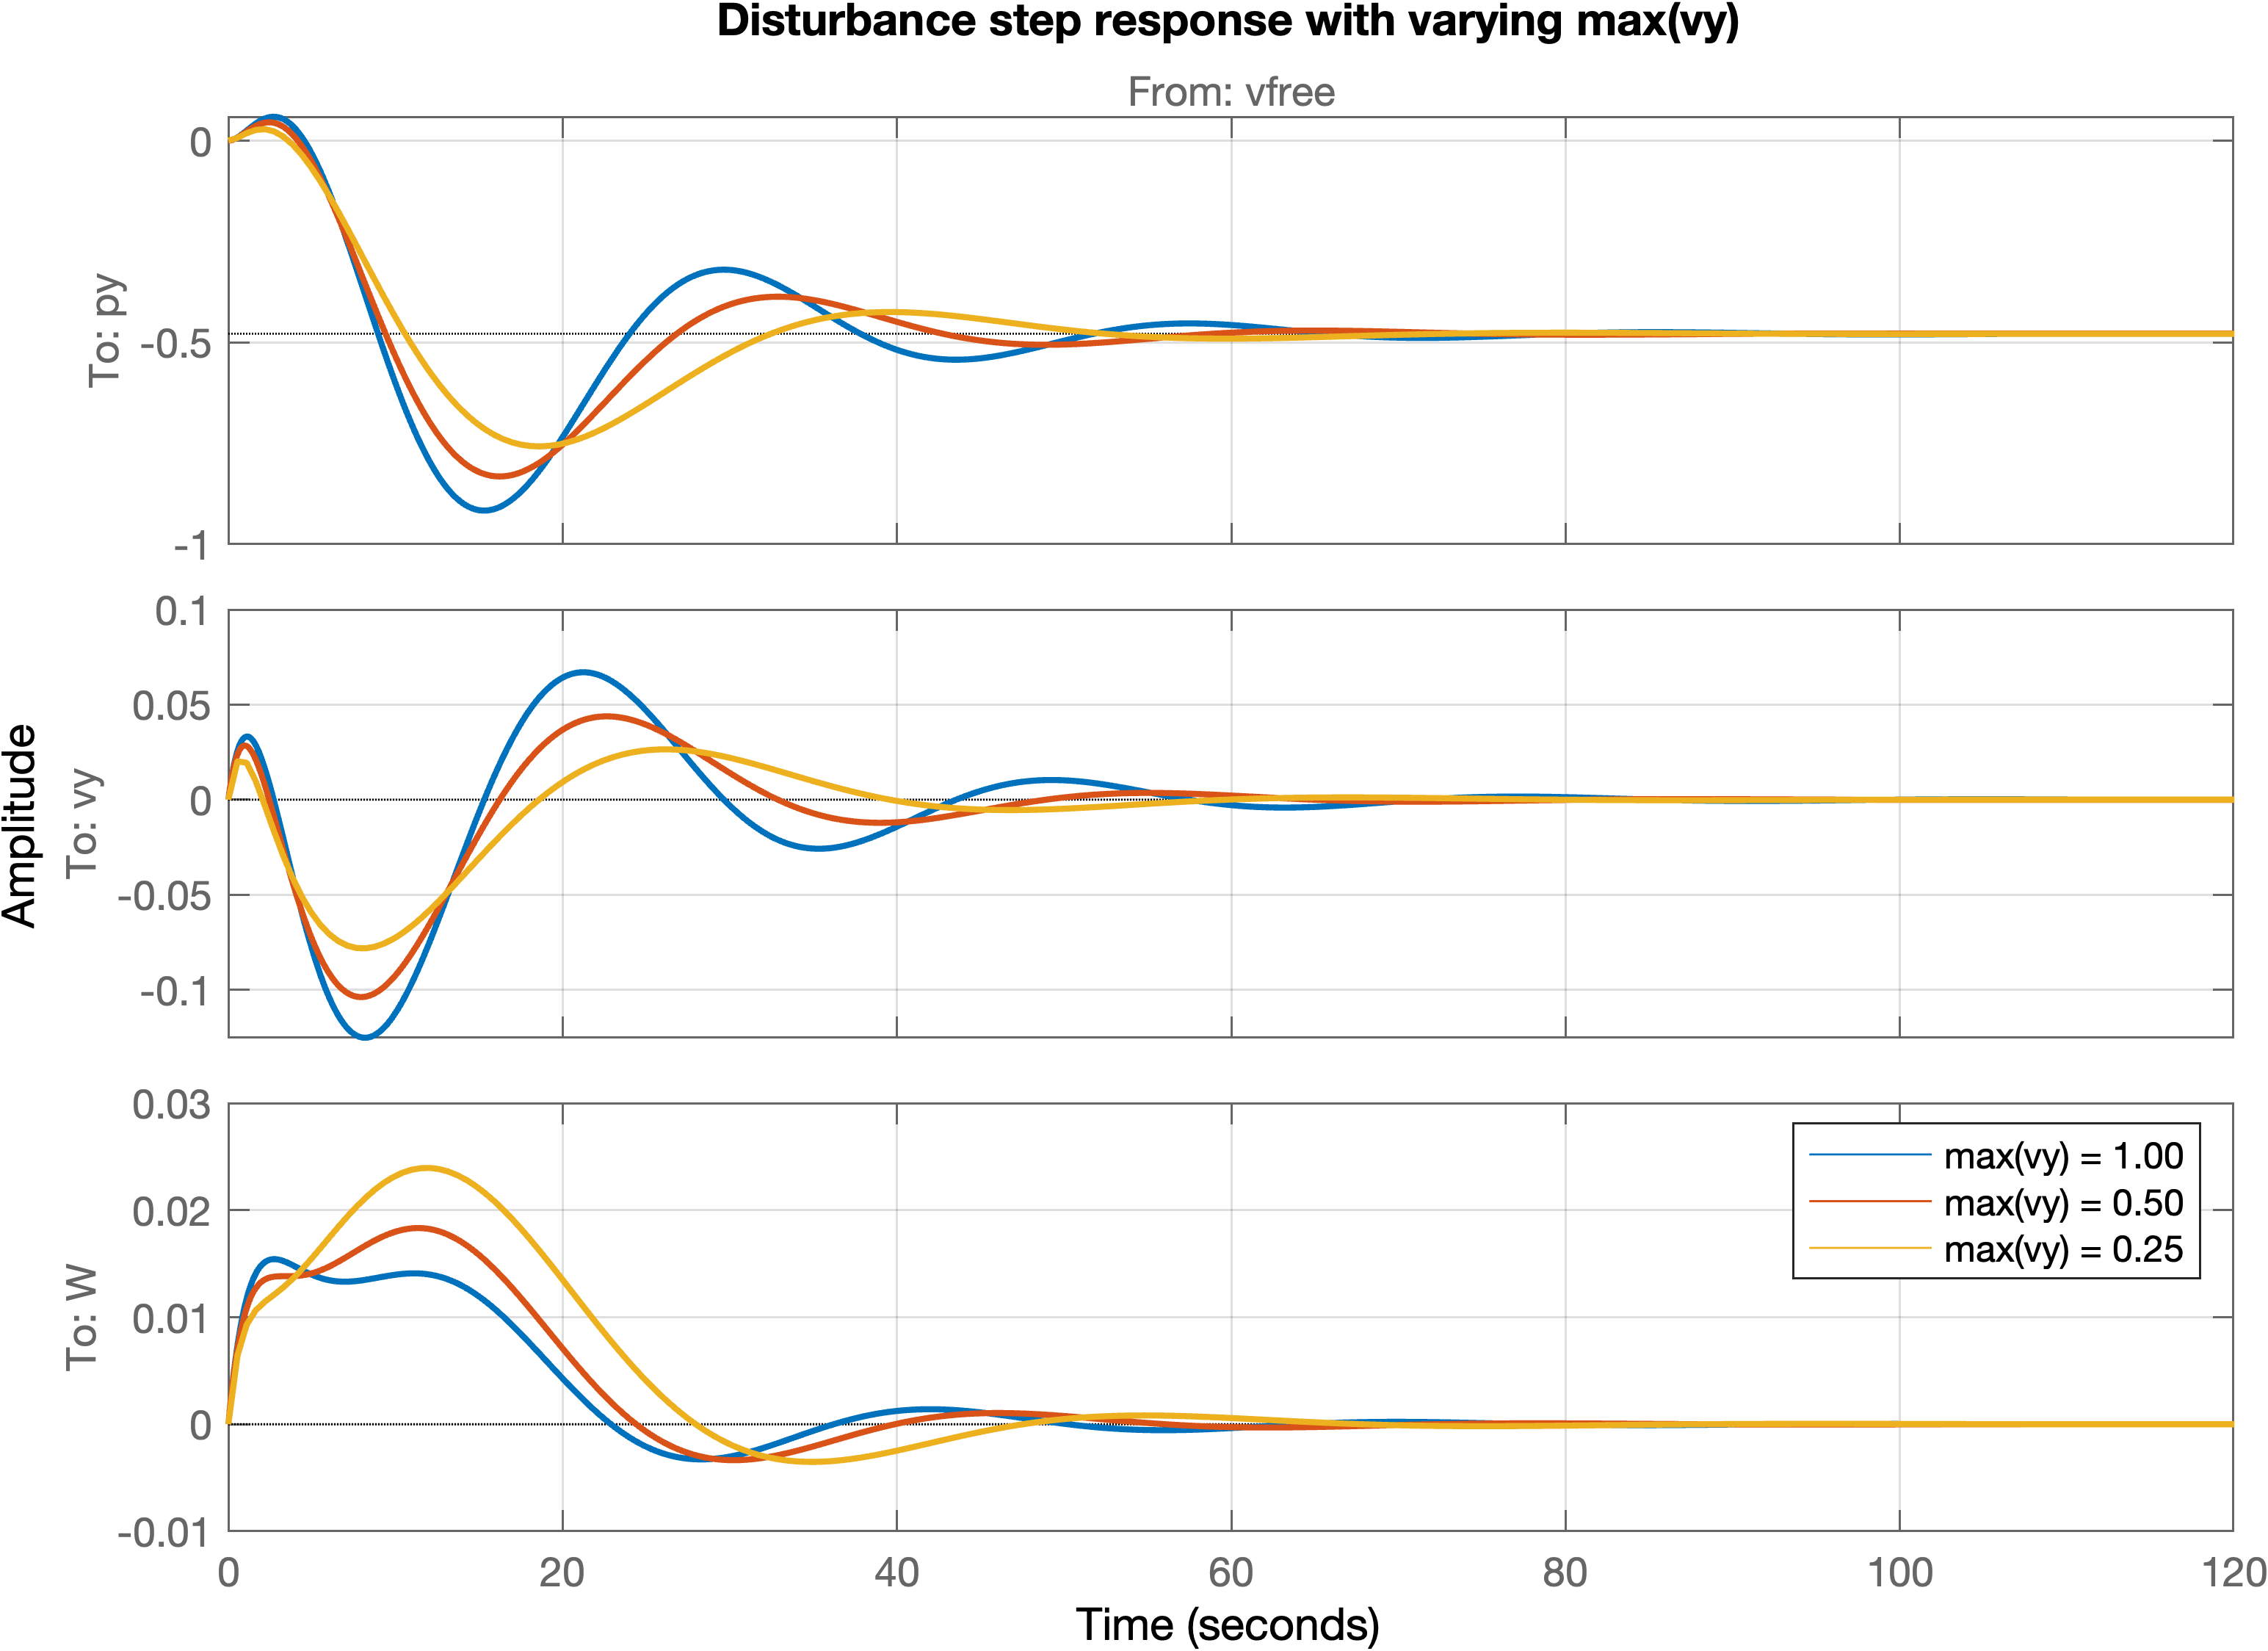
\includegraphics[width=0.7\textwidth]{Graphics/LQI pole zero/102_step_vy.png}
	\caption{Step response}
	\label{fig:step_vy}
\end{figure}



% OMEGA
\begin{figure*}[ht]
	\centering
	
	\subfloat[Pole-zero map]
	{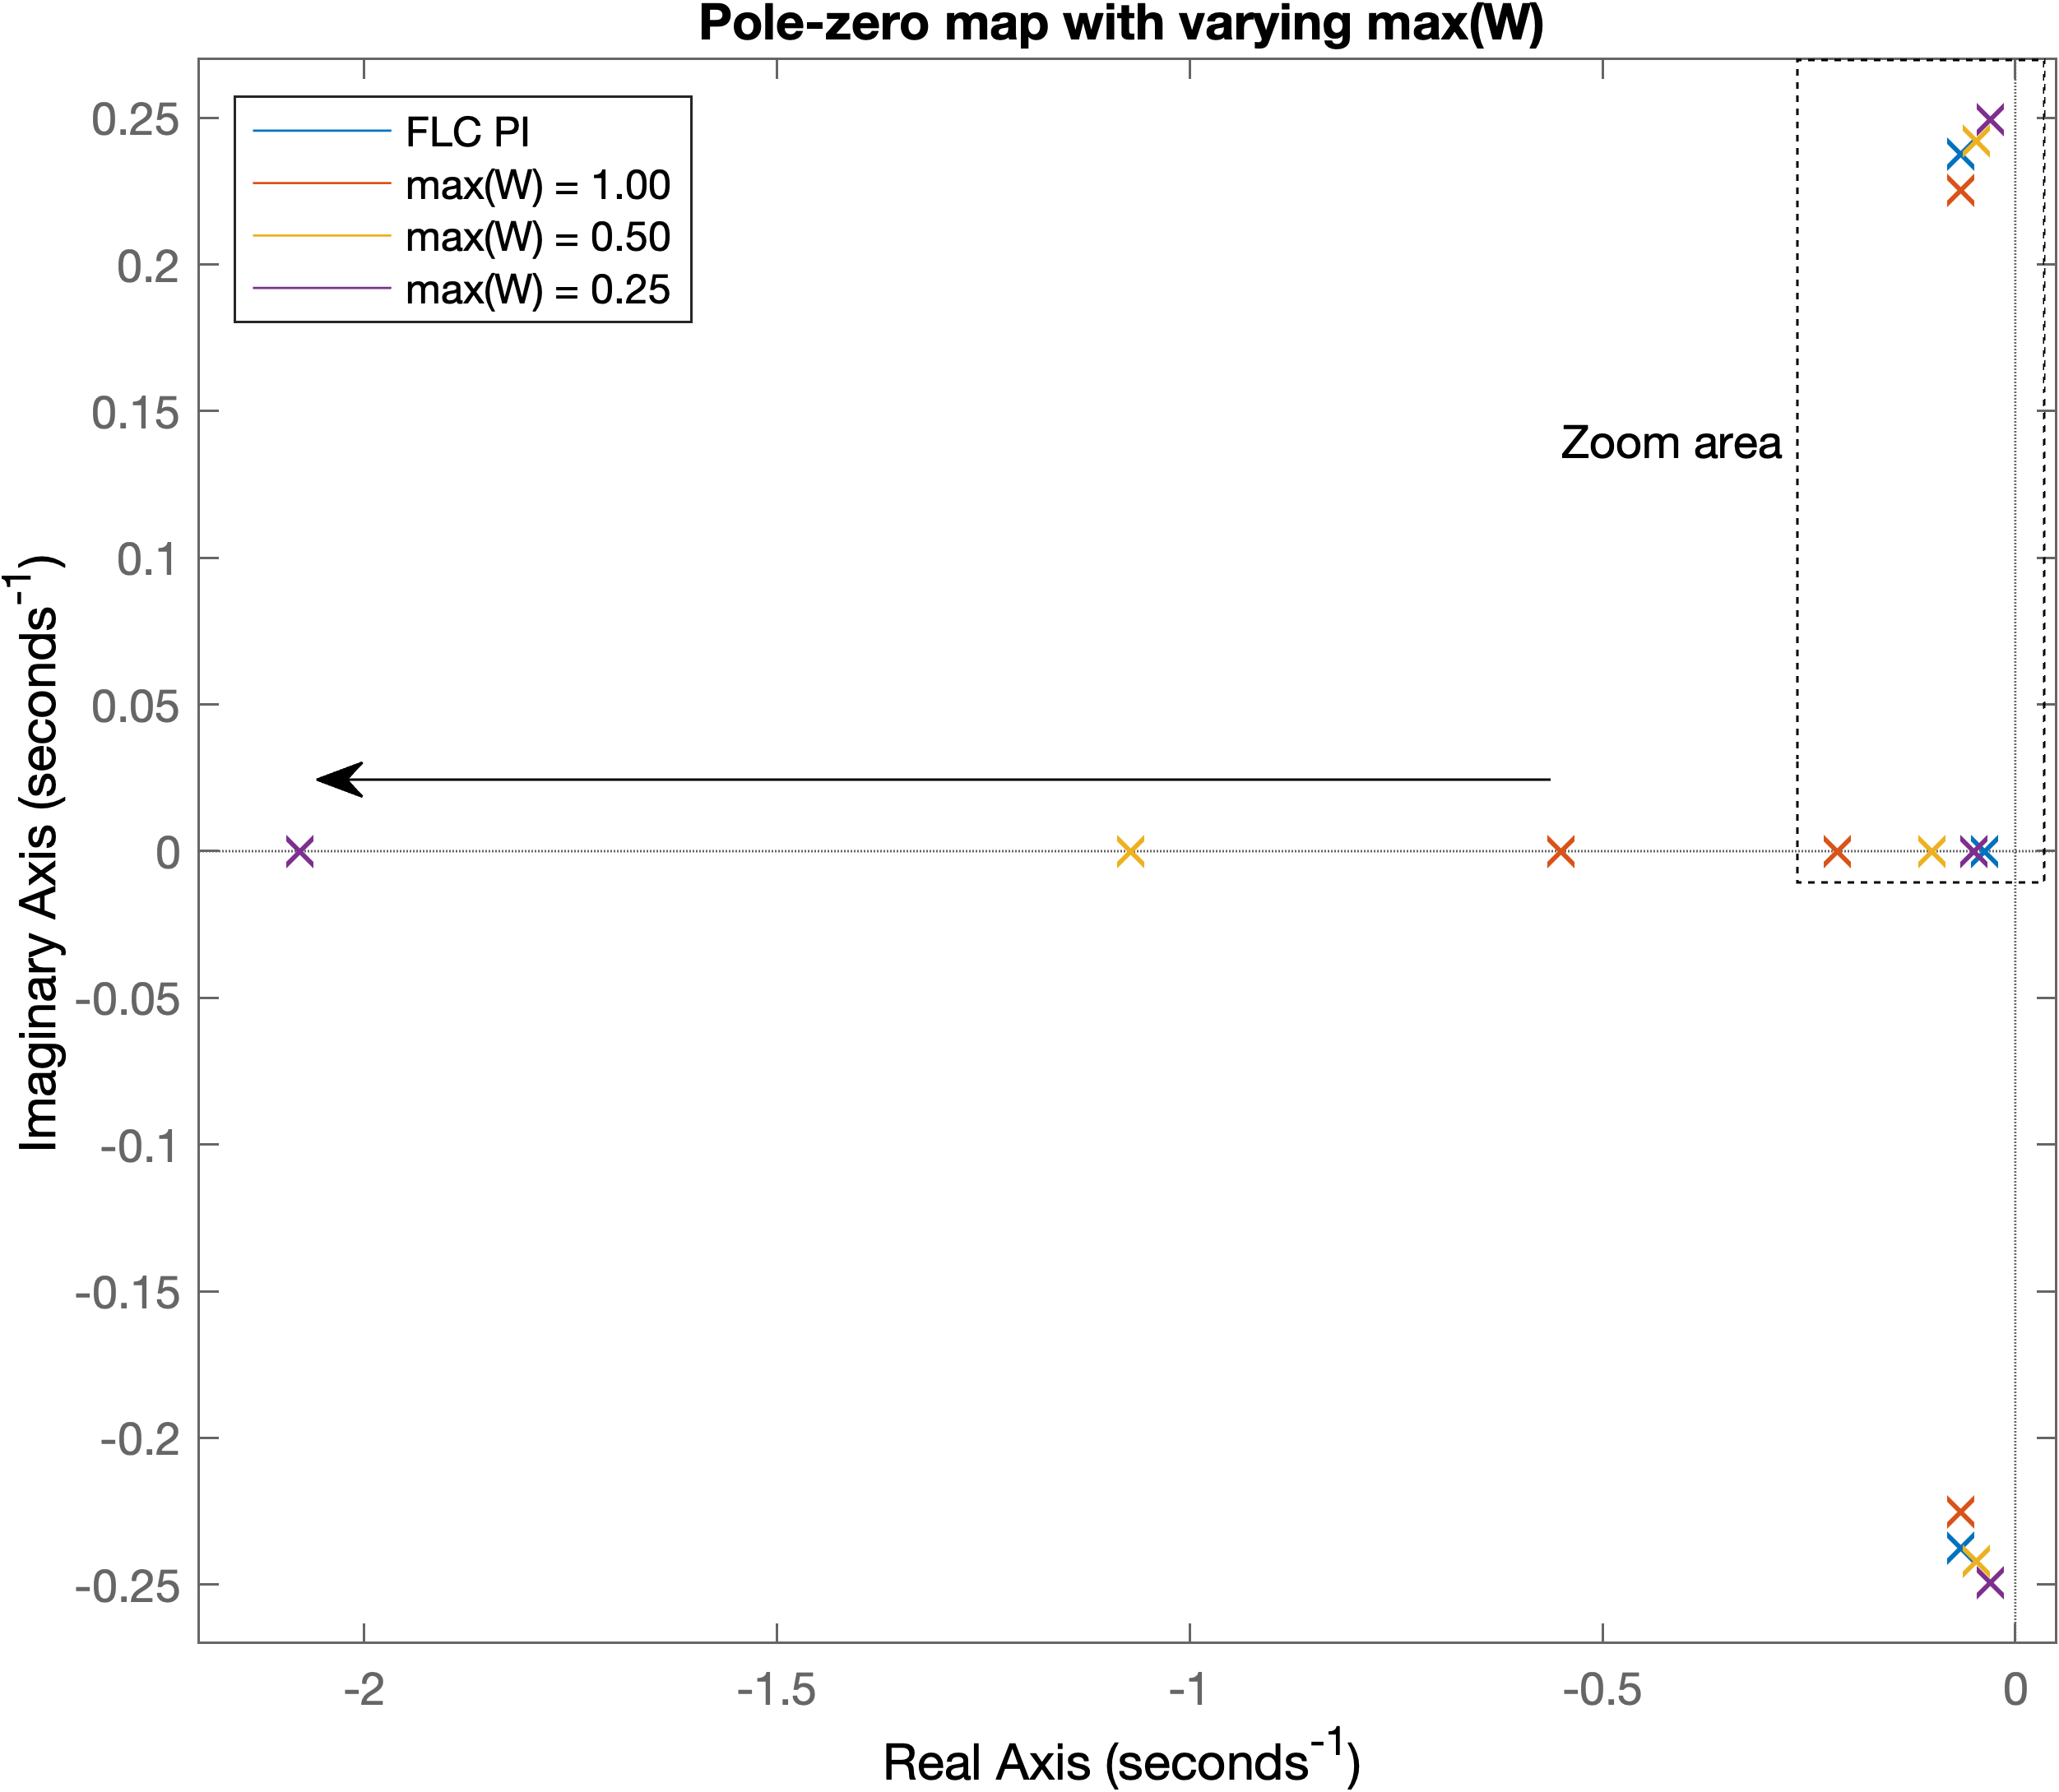
\includegraphics[width=.48\textwidth]{Graphics/LQI pole zero/03_pzmap_W}%
		\label{fig:pzmap_W}}
	\hfil
	\subfloat[Pole-zero map zoomed]
	{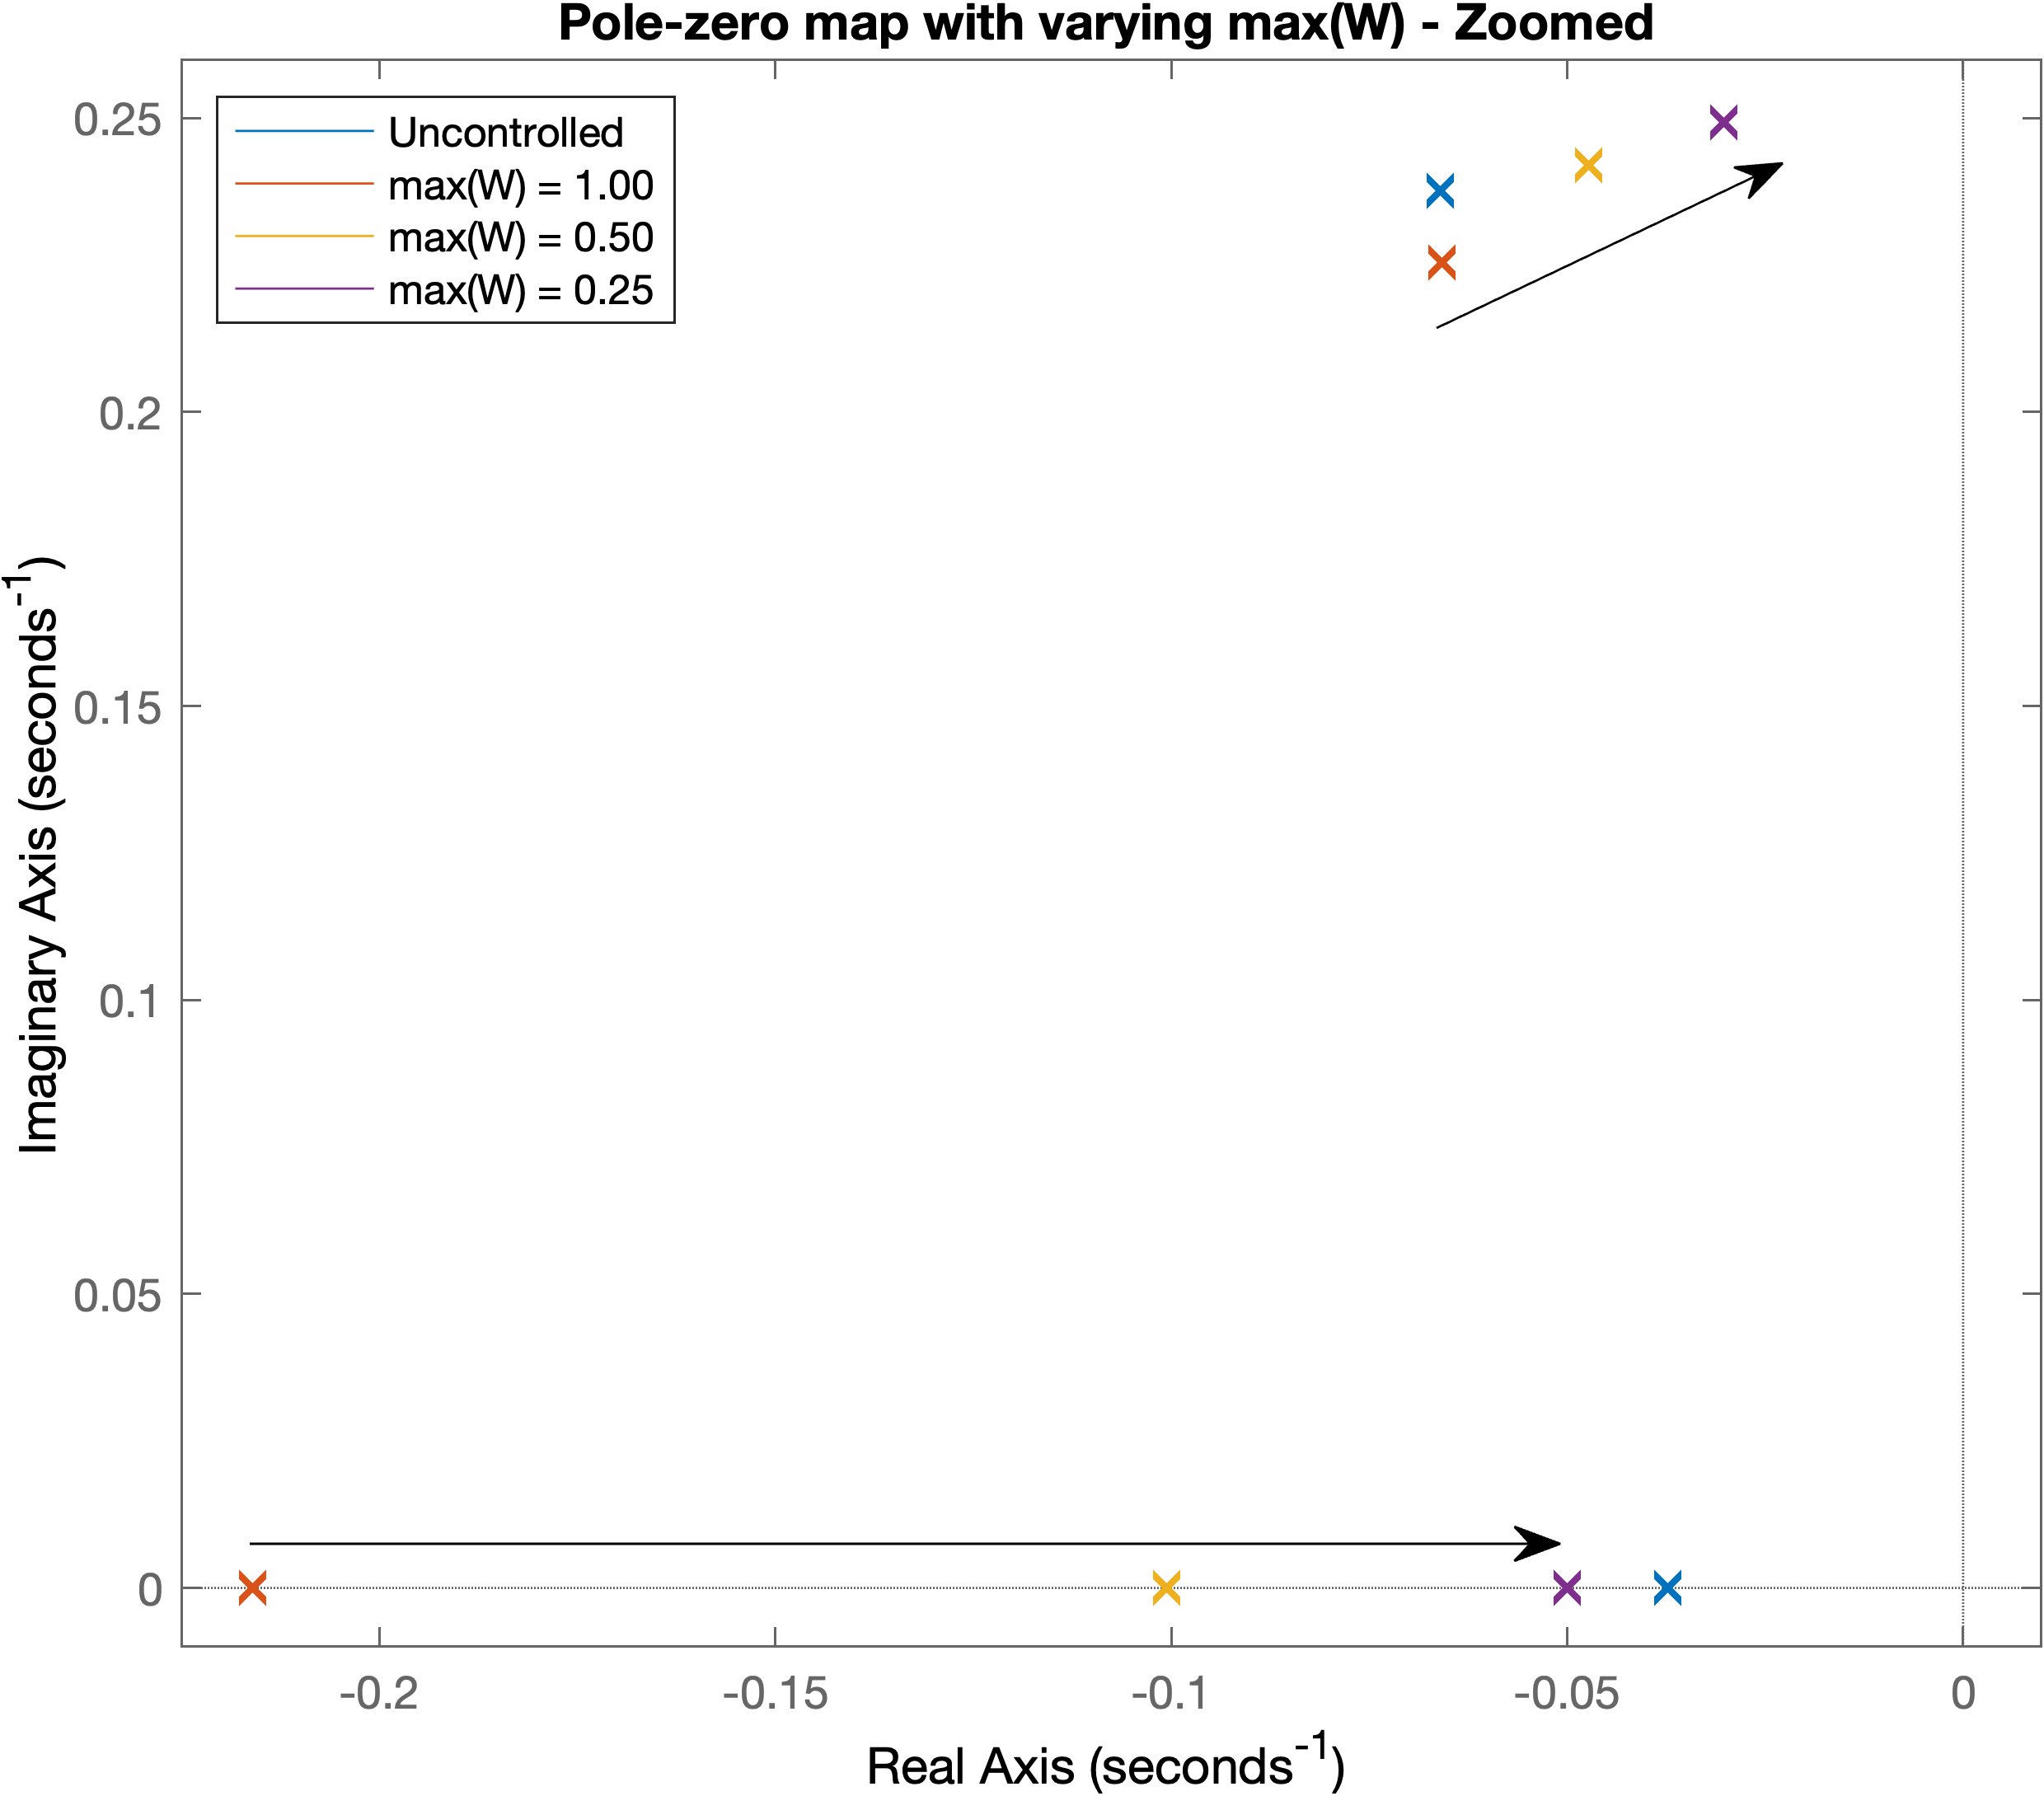
\includegraphics[width=.48\textwidth]{Graphics/LQI pole zero/13_pzmapzoom_W}%
		\label{fig:pzmap_W_zoom}}
	
	\caption{Pole-zero diagram with varying LQI weight of the state $ \Omega $; \textbf{(a)} a-text; \textbf{(b)} b-text.}
	\label{fig:pzmap_W_both}
\end{figure*}

\begin{figure}[ht]
	\centering
	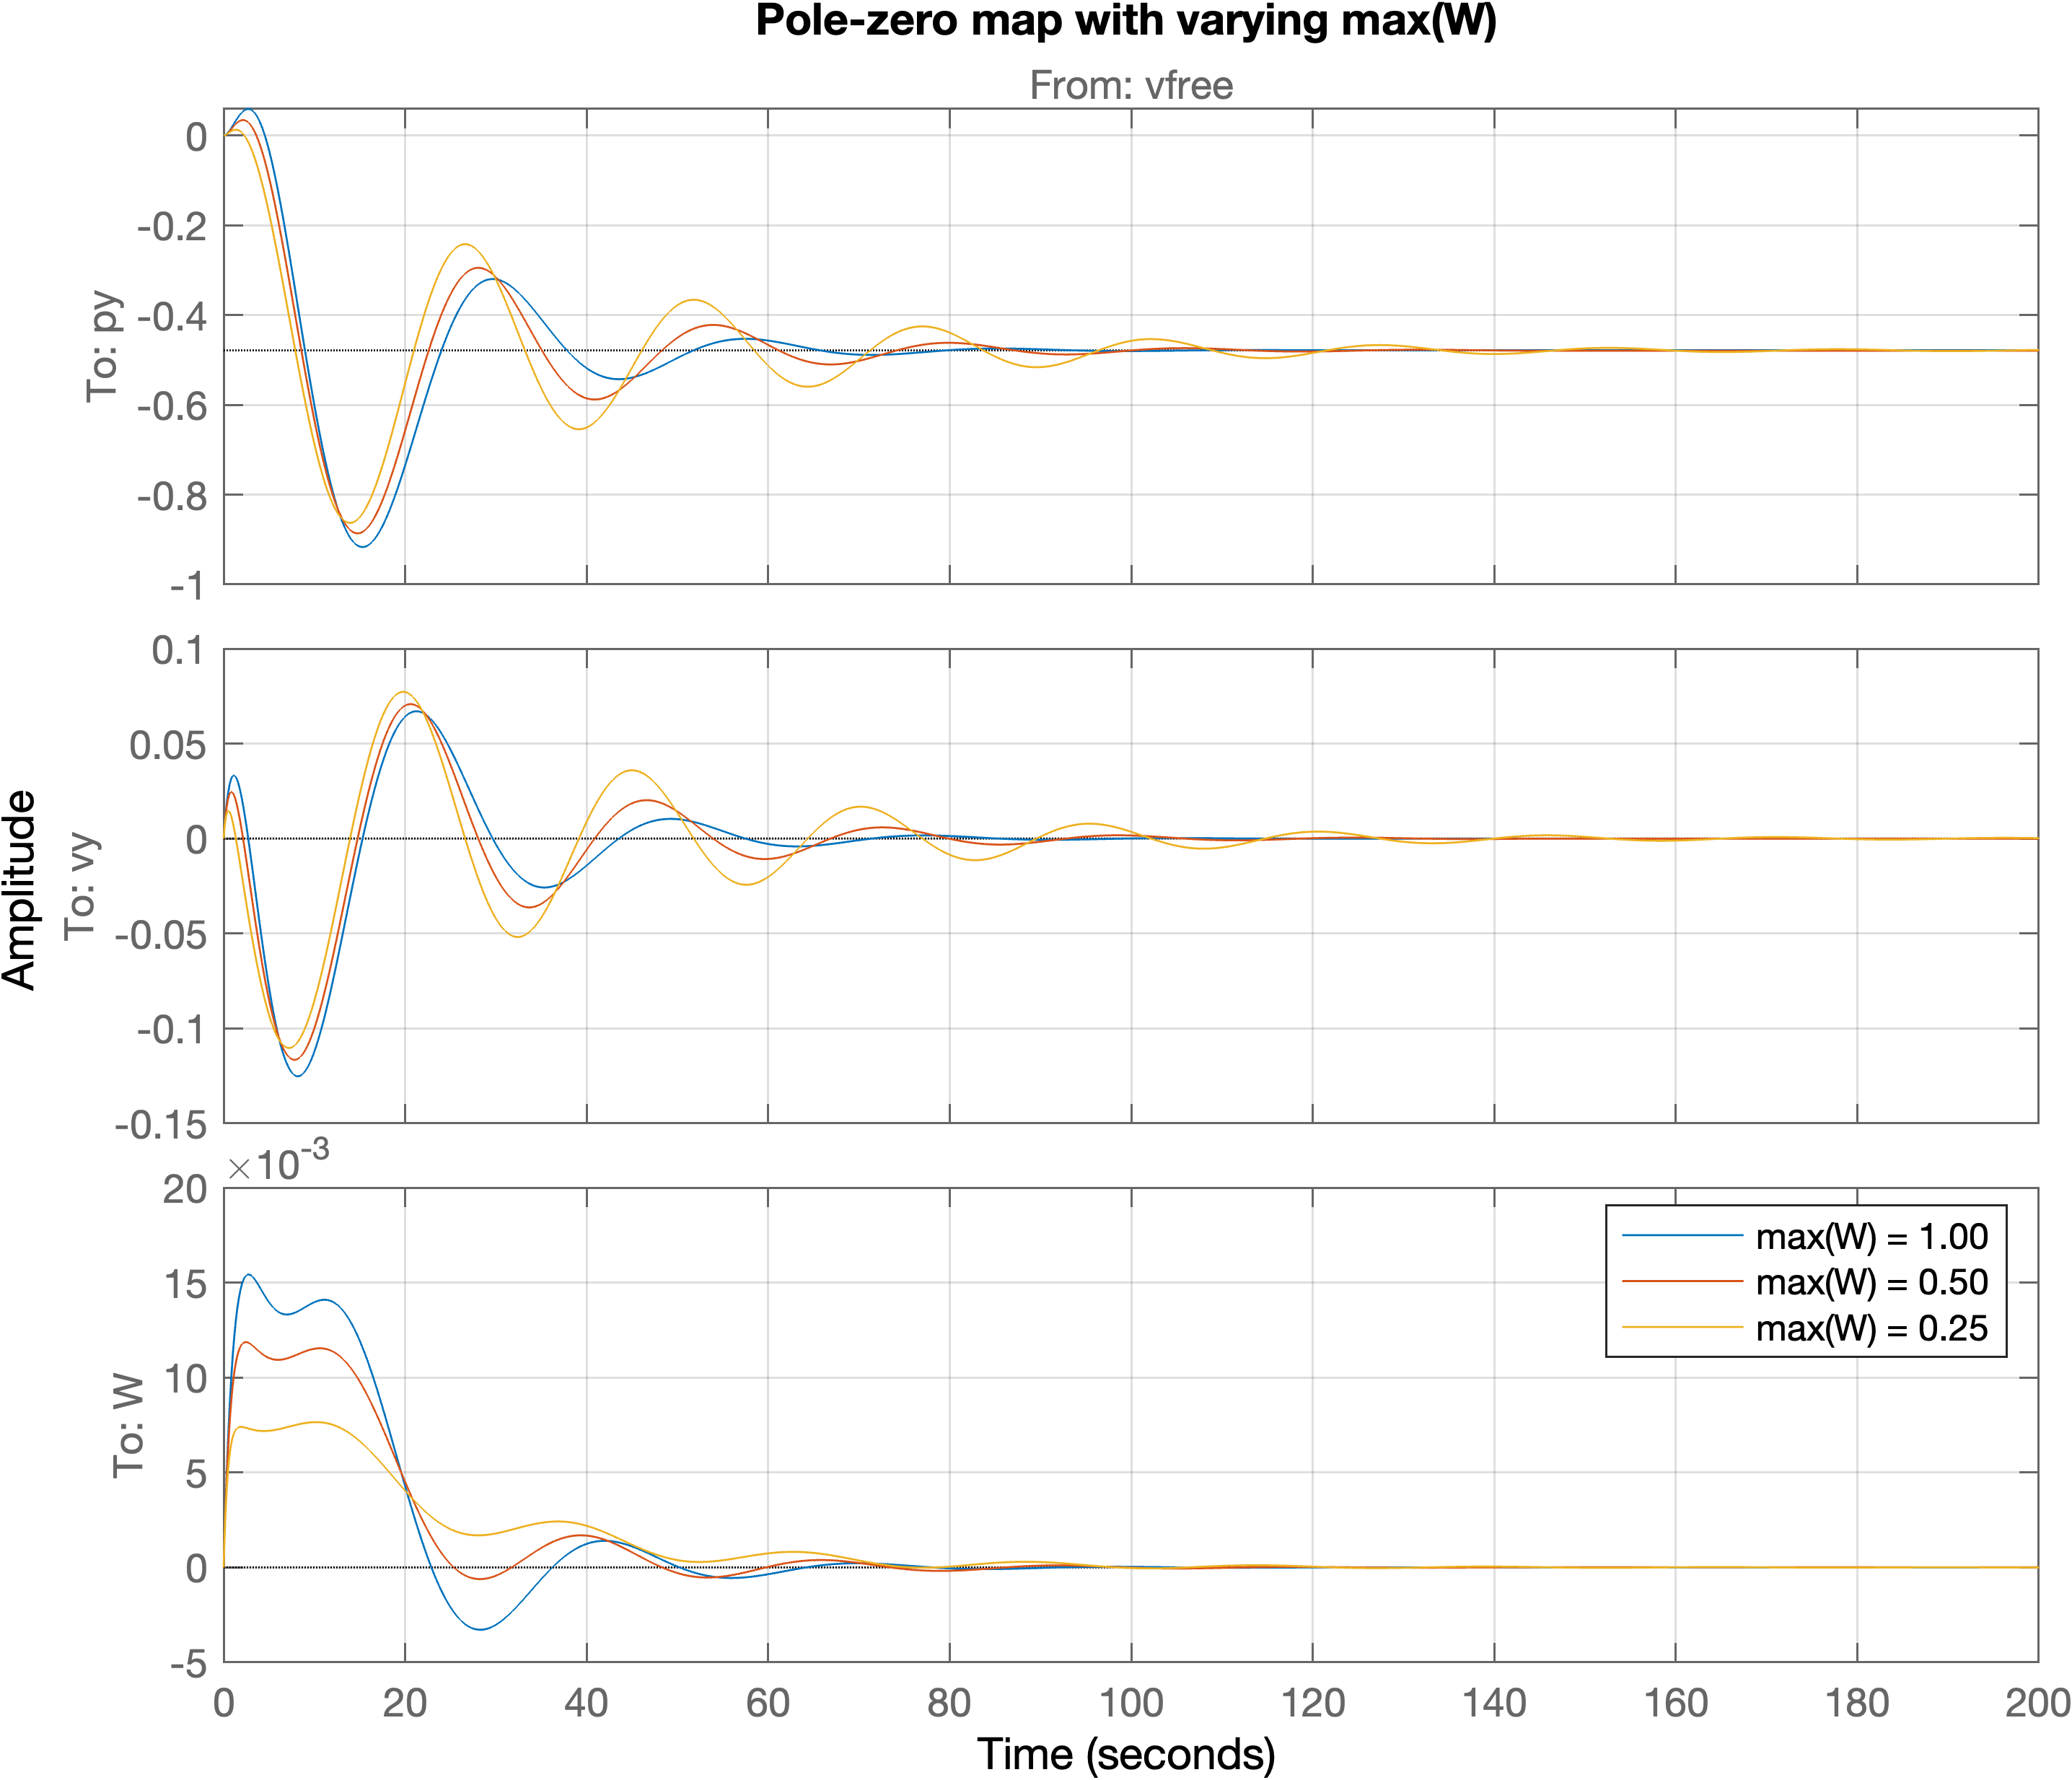
\includegraphics[width=0.7\textwidth]{Graphics/LQI pole zero/103_step_W.png}
	\caption{Step response}
	\label{fig:step_W}
\end{figure}

% THETA
\begin{figure}[ht]
	\centering
	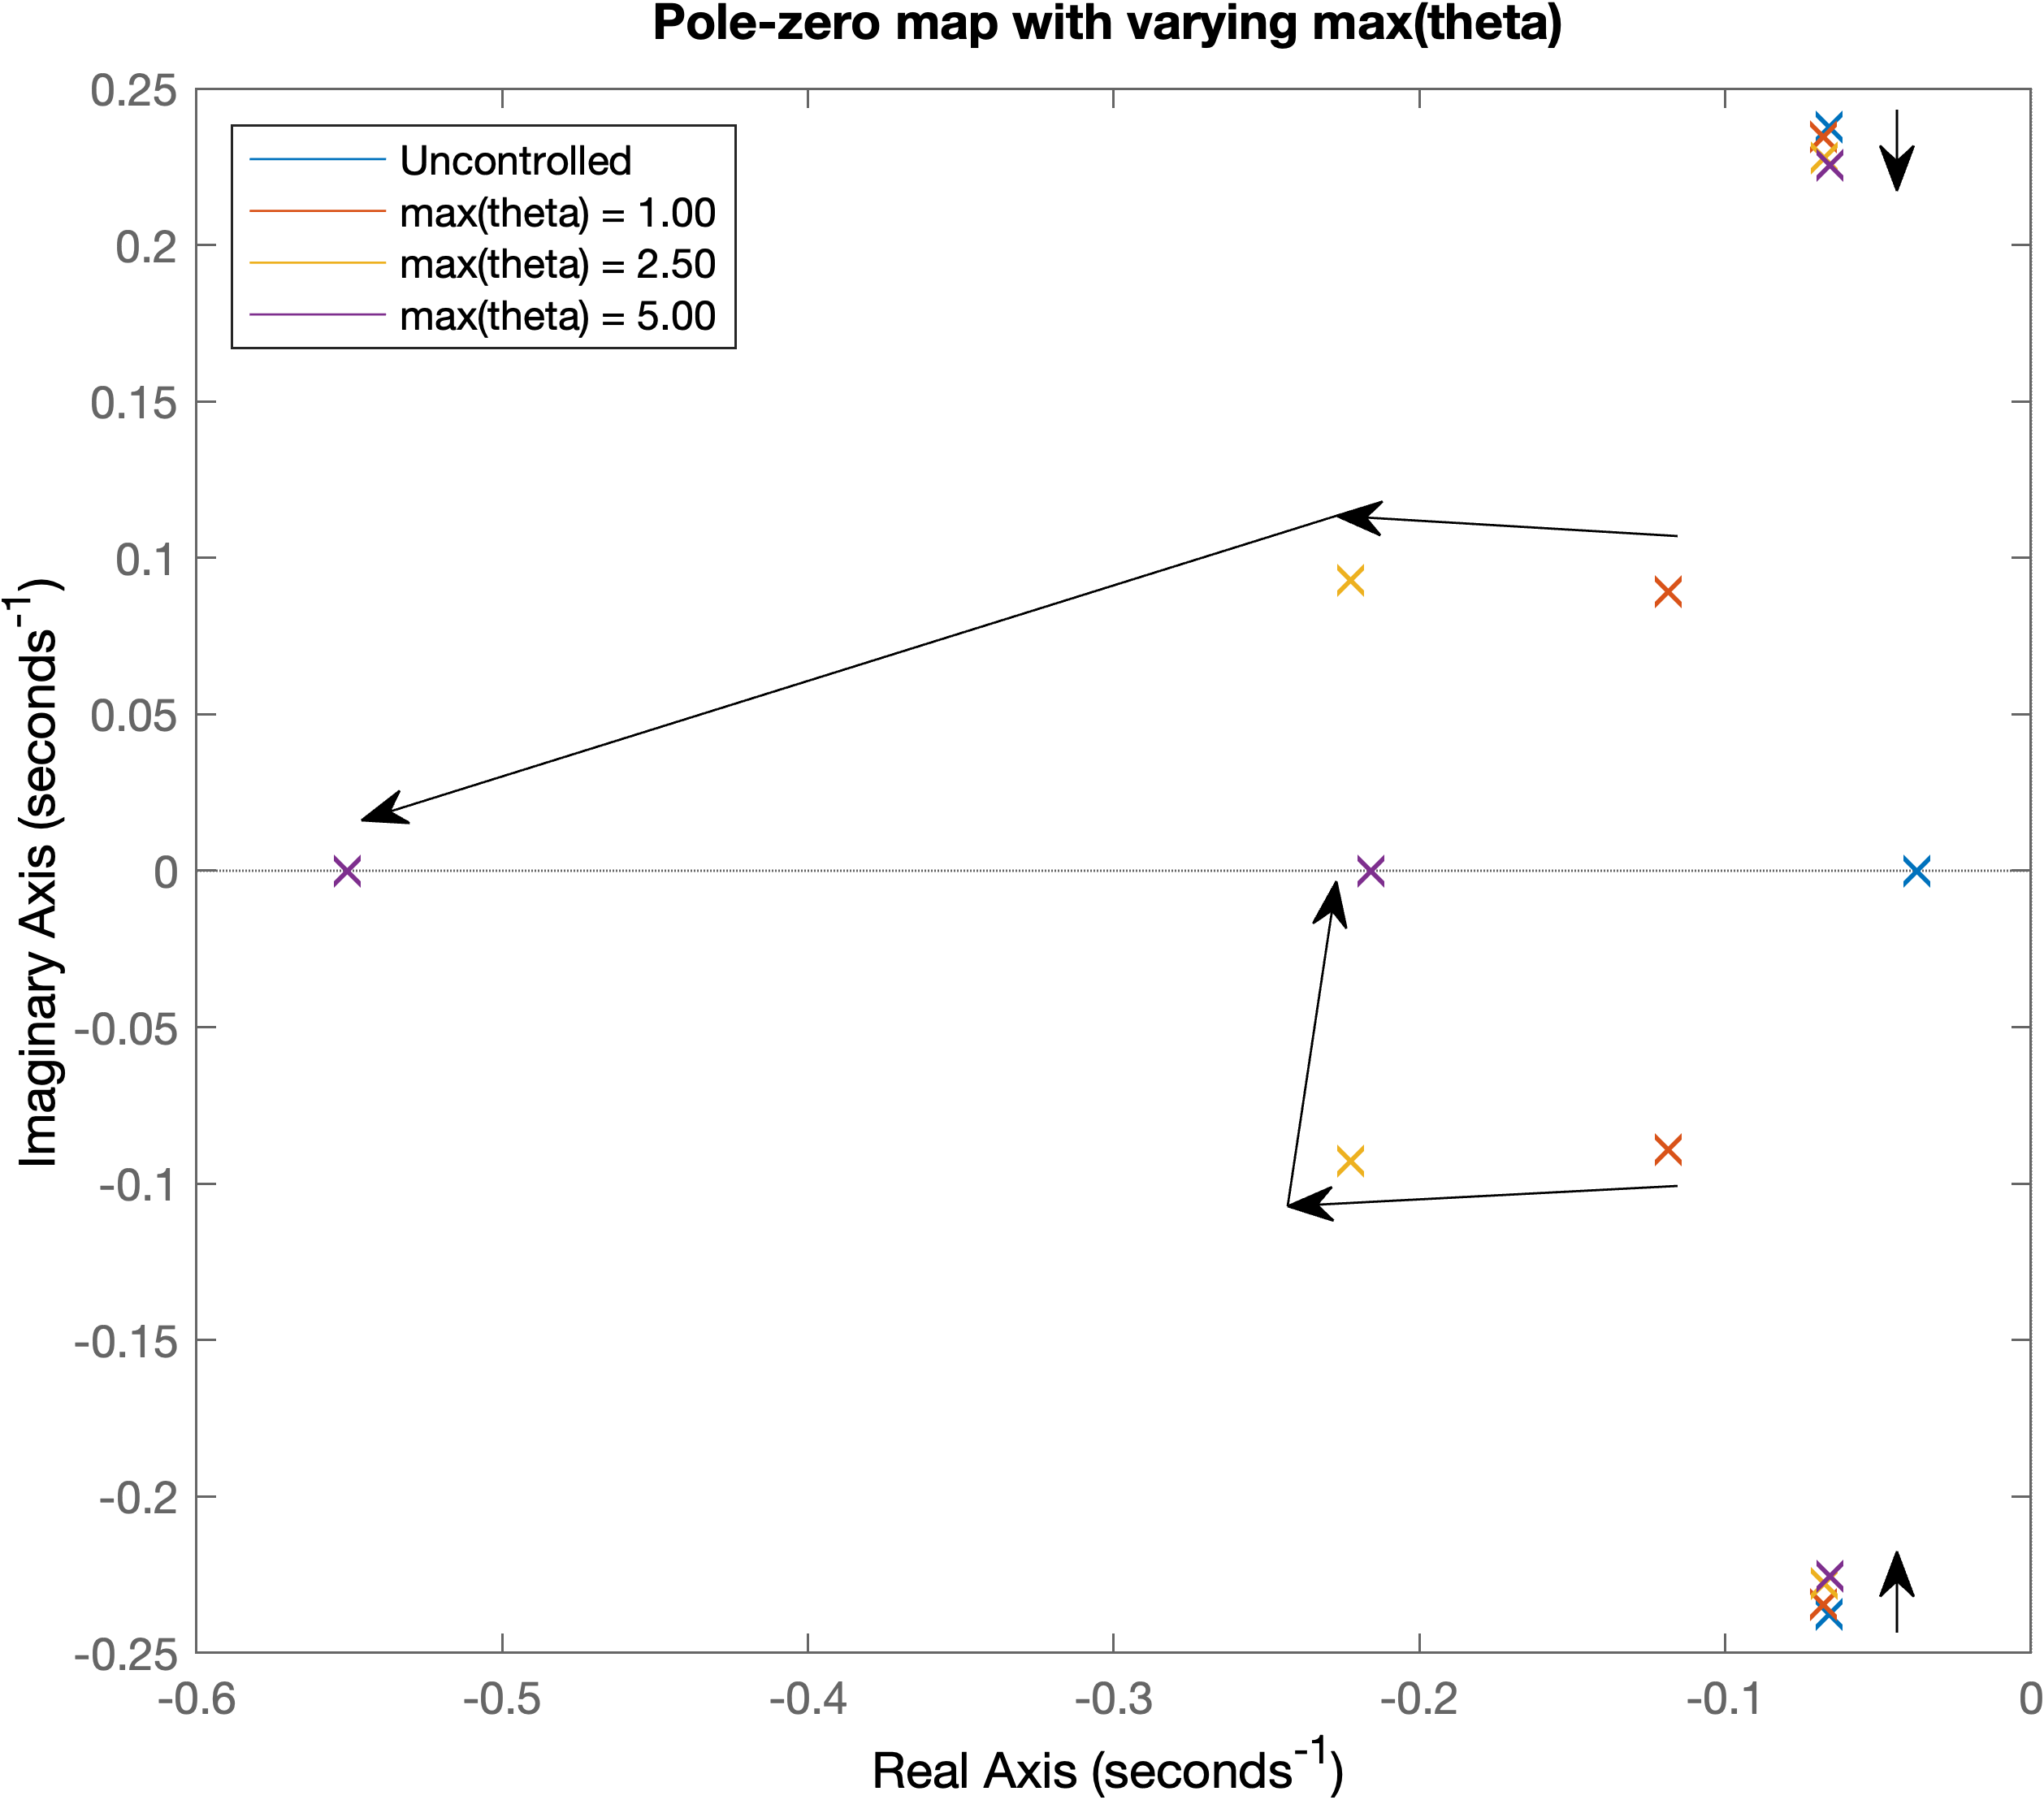
\includegraphics[width=0.55\textwidth]{Graphics/LQI pole zero/05_pzmap_theta.png}
	\caption{Poze-zero diagram with varying LQI weight on the actuator input $ \theta $}
	\label{fig:pzmap_theta}
\end{figure}

\begin{figure}[ht]
	\centering
	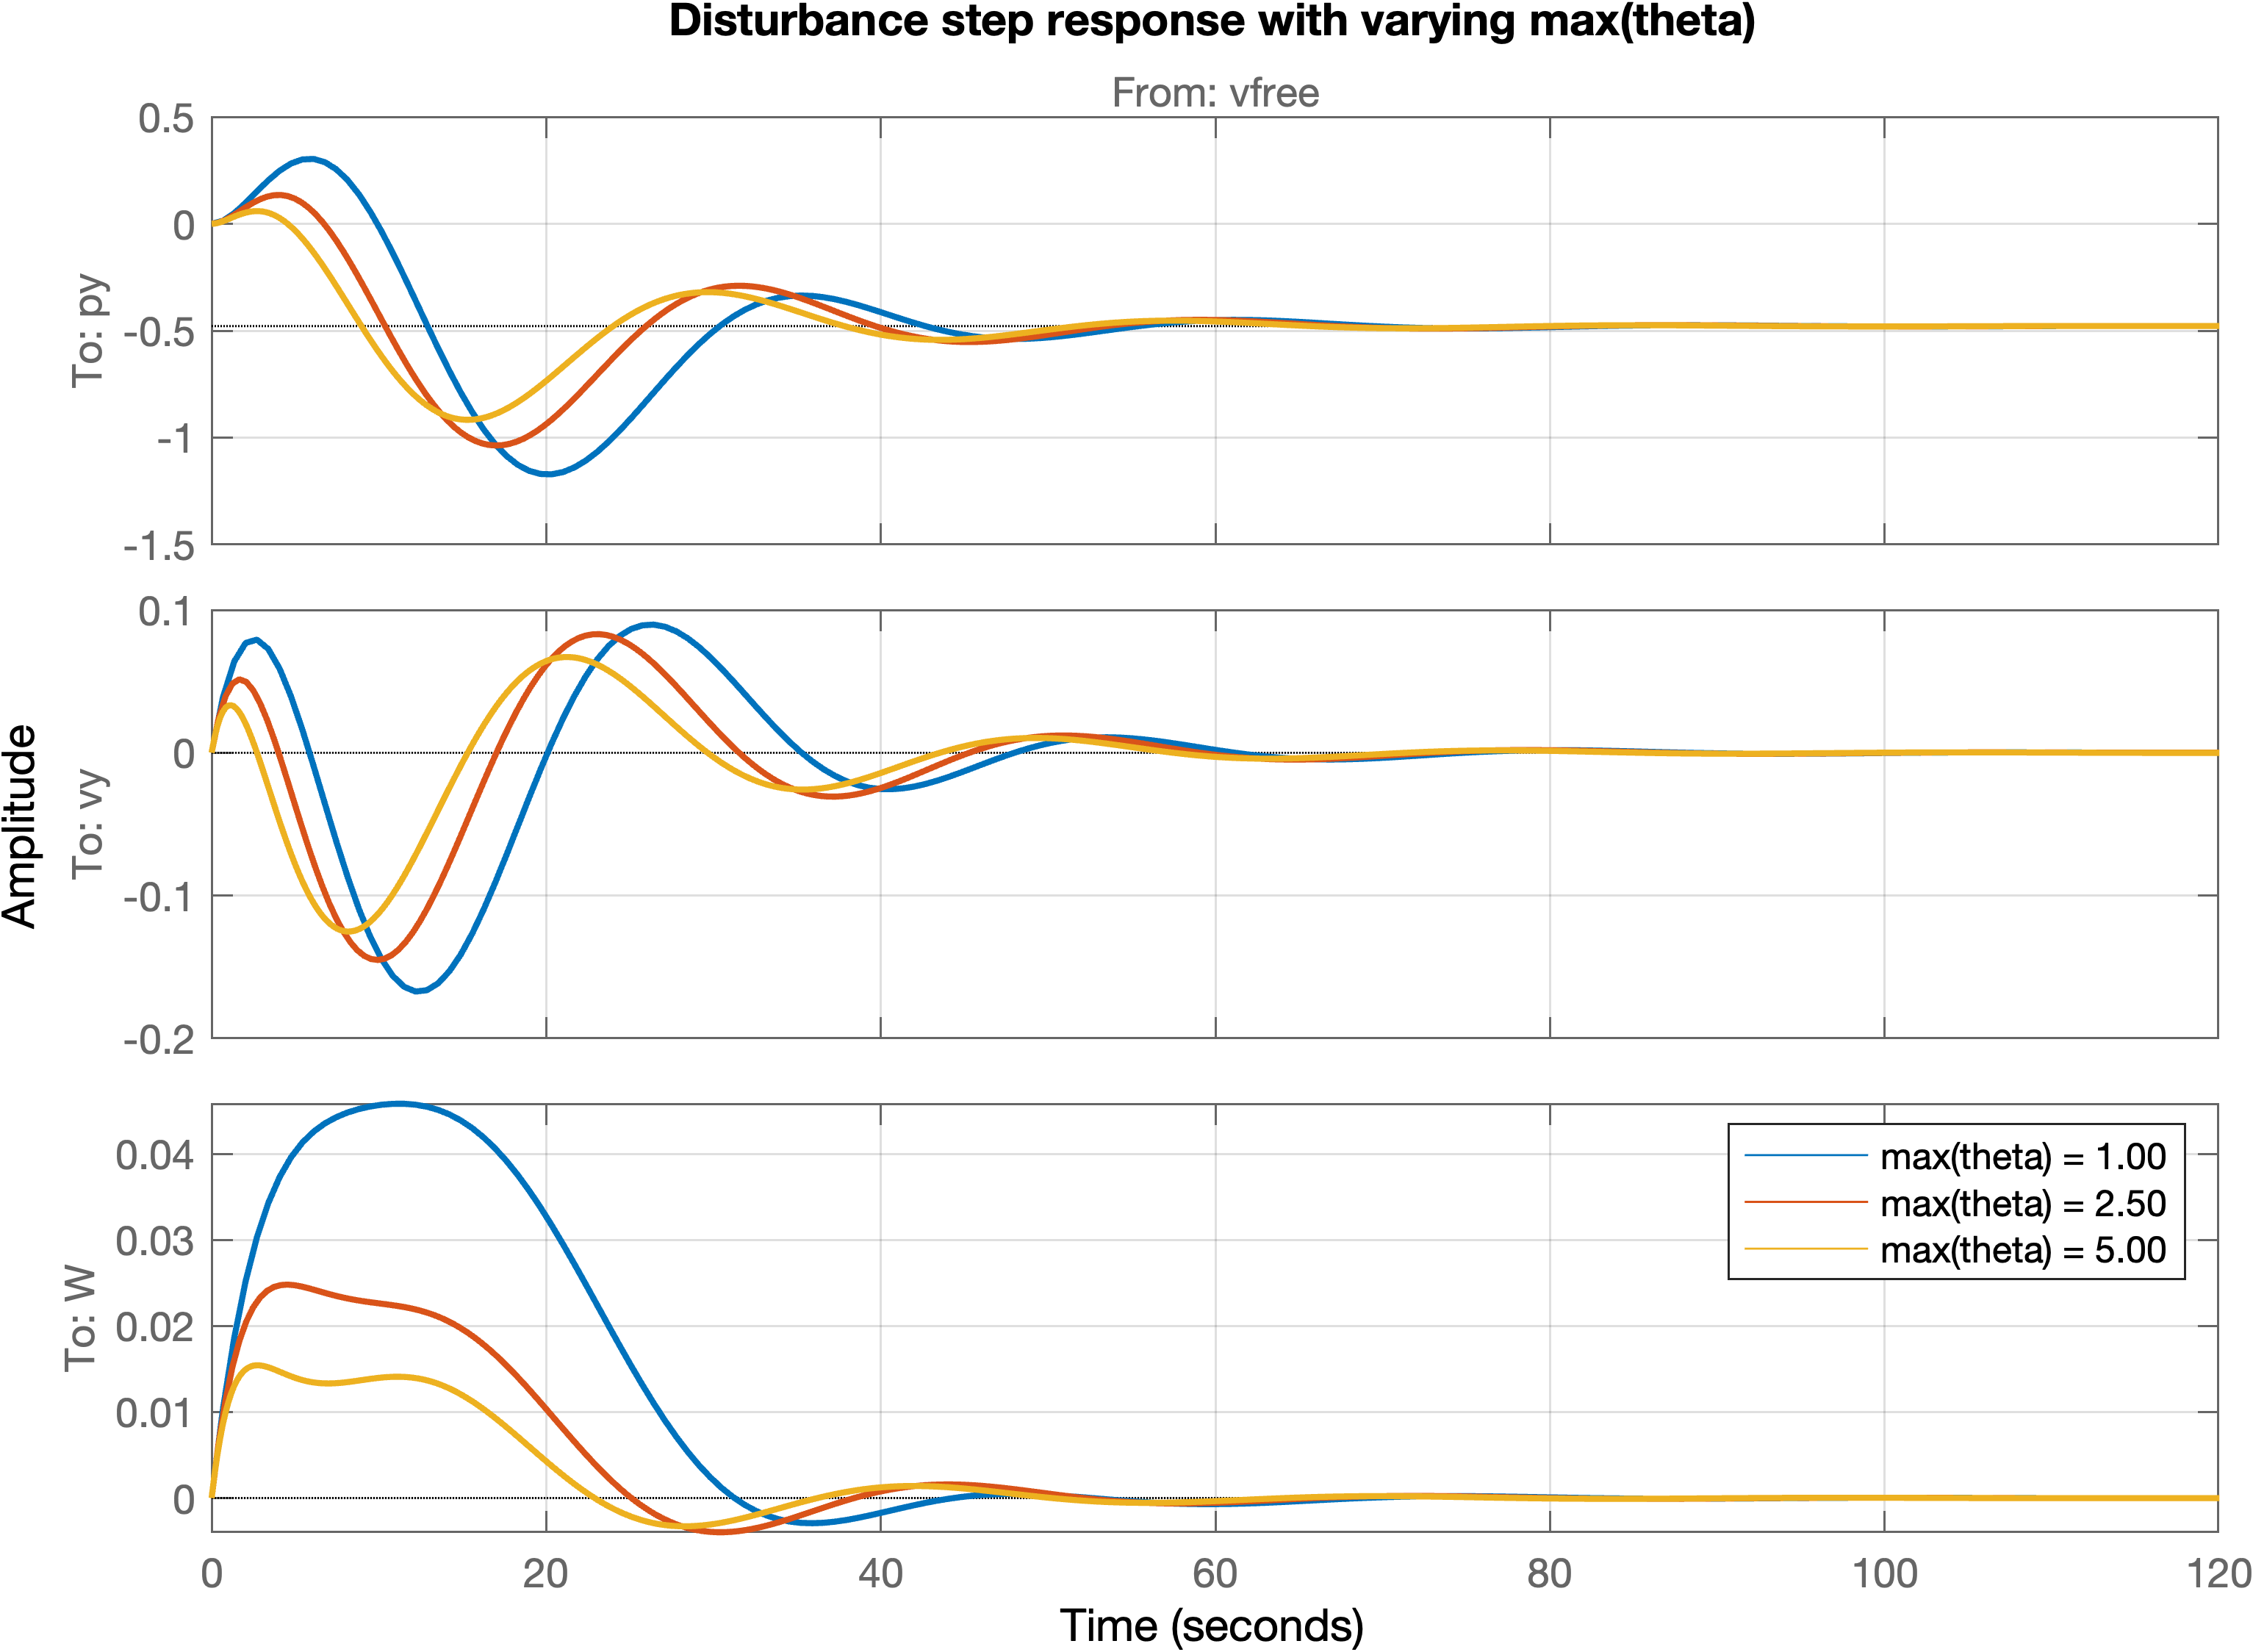
\includegraphics[width=0.7\textwidth]{Graphics/LQI pole zero/105_step_theta.png}
	\caption{Step response}
	\label{fig:step_theta}
\end{figure}

%\begin{figure*}[ht]
%	\centering
%	
%	\subfloat[sub-float1]
%	{\includegraphics[width=.49\textwidth]{Graphics/LQI pole zero/}%
%		\label{fig:1}}
%	\hfil
%	\subfloat[sub-float2]
%	{\includegraphics[width=.50\textwidth]{Graphics/LQI pole zero/}%
%		\label{fig:2}}
%	
%	\caption{Total text; \textbf{(a)} a-text; \textbf{(b)} b-text.}
%	\label{fig:3}
%\end{figure*}